\question{Câu 7}

Cho mạch khuếch đại tín hiệu như hình vẽ, BJT $Q_{1}$ có hệ số $\beta = 50$ và $Q_{2}$ có hệ số $\beta = 100$. Các hệ số $V_{A} = \infty$.

\begin{figure}[H]
	\centering
	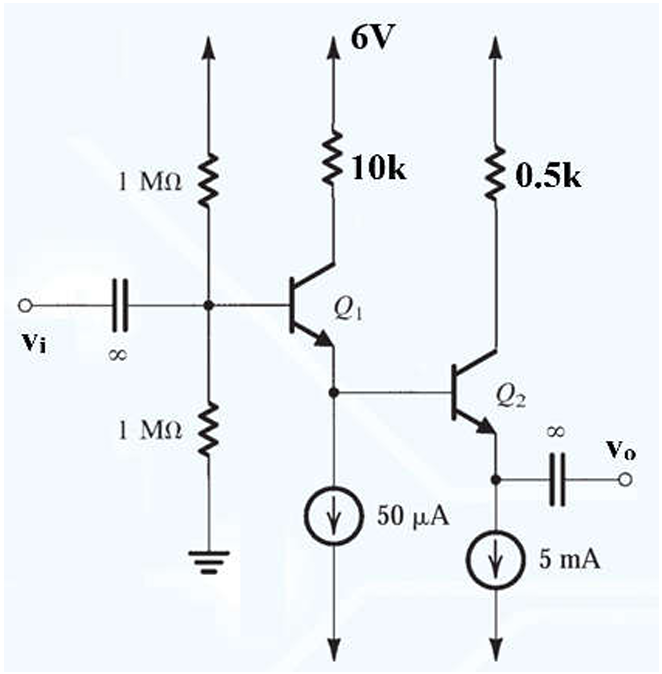
\includegraphics[width=\linewidth]{./my-chapters/my-images/Question7/debai.png}
\end{figure}

\answer{a}{Tìm điểm hoạt động $Q_{1}$ và $Q_{2}$ của BJT.}

\begin{itemize}[label=-]
	\item Sweep BJT $Q_{2}$ để tìm được điện áp $V_{BE2}$
	
	\begin{figure}[H]
		\centering
		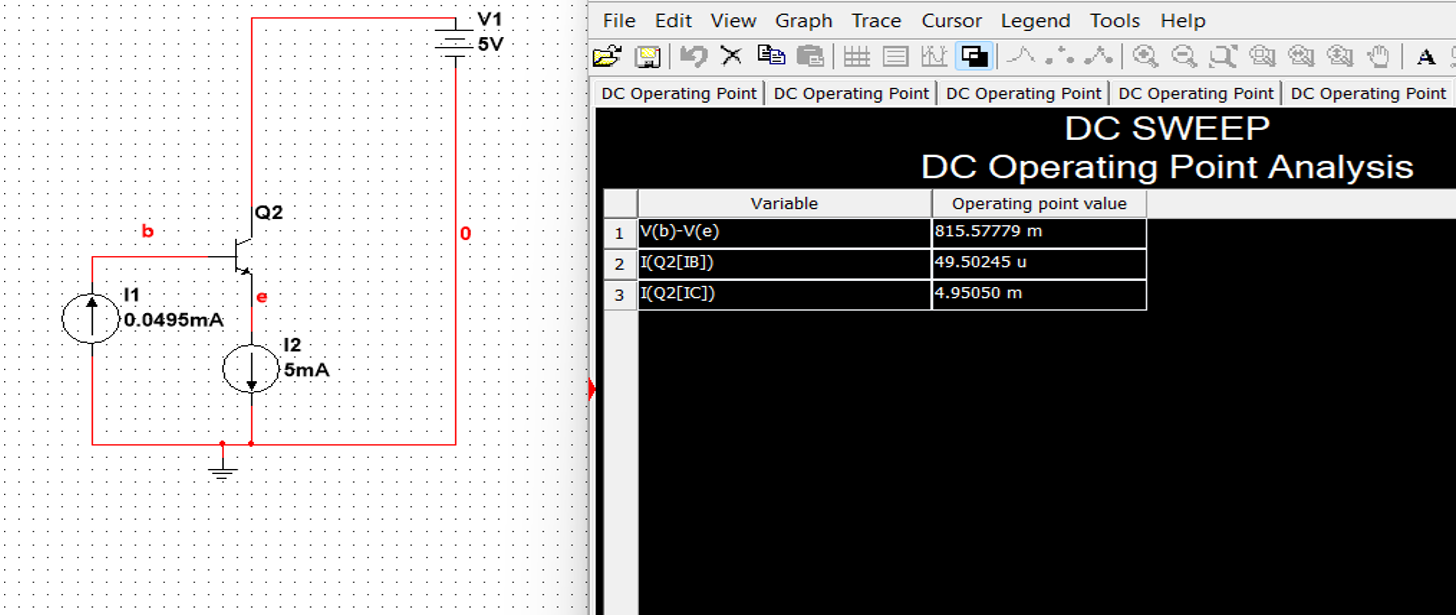
\includegraphics[width=.8\linewidth]{./my-chapters/my-images/Question7/a_quetVbe_q2.png}
	\end{figure} 
	
	\begin{itemize}[label=-, leftmargin=1cm]
		\item $I_{B2} = \dfrac{I_{E2}}{\beta_{2} + 1} = \dfrac{5\,\textsf{m}}{101} = 0.0495\,\textsf{mA}$
		
		$\Rightarrow I_{C2} = \beta I_{B2} = 100\times 0.0495 = 4.95\,\textsf{mA}$
	\end{itemize}
	
	\item Sweep BJT $Q_{1}$ để tìm được điện áp $V_{BE1}$
	
	\begin{figure}[H]
		\centering
		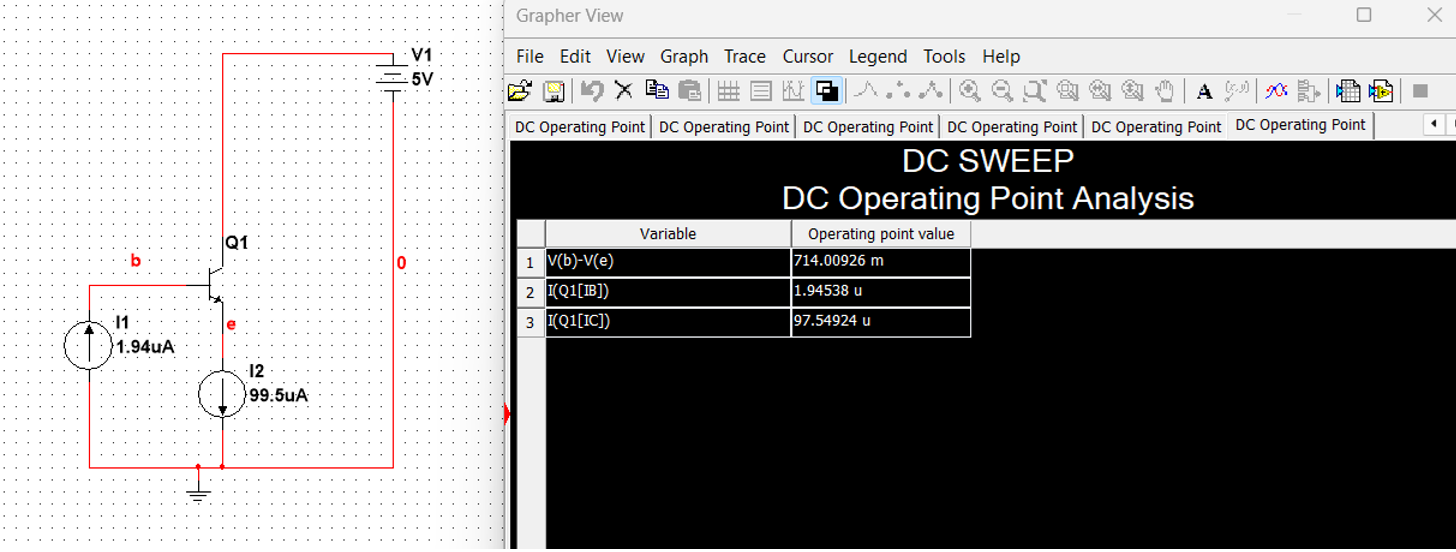
\includegraphics[width=.8\linewidth]{./my-chapters/my-images/Question7/a_quetVbe.png}
	\end{figure} 
	
	\begin{itemize}[label=-, leftmargin=1cm]
		\item $I_{E1} = I_{B2} + 50\mu\textsf{A} = 49.5\mu + 50\mu = 99.5\mu\textsf{A}$
		
		$\Rightarrow I_{C1} = \dfrac{I_{E1}}{\beta_{1} + 1}\beta_{1} = \dfrac{99.5}{51}\times 50 = 97\mu\textsf{A}$
		
		$\Rightarrow I_{B1} = \dfrac{I_{C1}}{\beta_{1}} = \dfrac{97}{50} = 1.94\mu\textsf{A}$
	\end{itemize}
\end{itemize}

Với, 
\[ R_{th} = R_{1} // R_{2} = 0.5\,\textsf{M}\Omega \]
\[ V_{th} = \dfrac{R_{2}}{R_{1} + R_{2}}\times 2V_{cc} - V_{cc} = \dfrac{1}{2}\times 2 \times 6 - 6 = 0\,\textsf{V} \]
\[ V_{B1} = V_{th} - R_{th}I_{B1} = 0 - 0.5\times 1.94 = -0.97\,\textsf{V}\]
\[ V_{E1} = V_{B1} - V_{BE1} = -0.97 - 0.714 = -1.684\,\textsf{V} \Rightarrow V_{E2} = V_{E1} - V_{BE2} = -1.684-0.816 = -2.5\,\textsf{V} \]
\[ \Rightarrow V_{CE1} = V_{cc} - I_{C1}R_{C1} - V_{E1} = 6 - 97\textsf{m}\times 10 - (- 1.684) = 6.714\,\textsf{V}\]
\[ \Rightarrow V_{CE2} = V_{cc} - I_{C2}R_{C2} - V_{E2} = 6-4.95\textsf{m}\times 0.5 - (- 2.5) = 6.025\,\textsf{V}\]

$\Rightarrow$ \finalresult{Q_{1}(I_{CQ1}\textsf{, }V_{CEQ1}) = (96\,\mu\textsf{A, } 6.714\,\textsf{V})} và \finalresult{Q_{2}(I_{CQ2}\textsf{, }V_{CEQ2}) = (4.95\,\textsf{mA, } 6.025\,\textsf{V})}.

Kiểm tra kết quả

\begin{figure}[H]
	\centering
	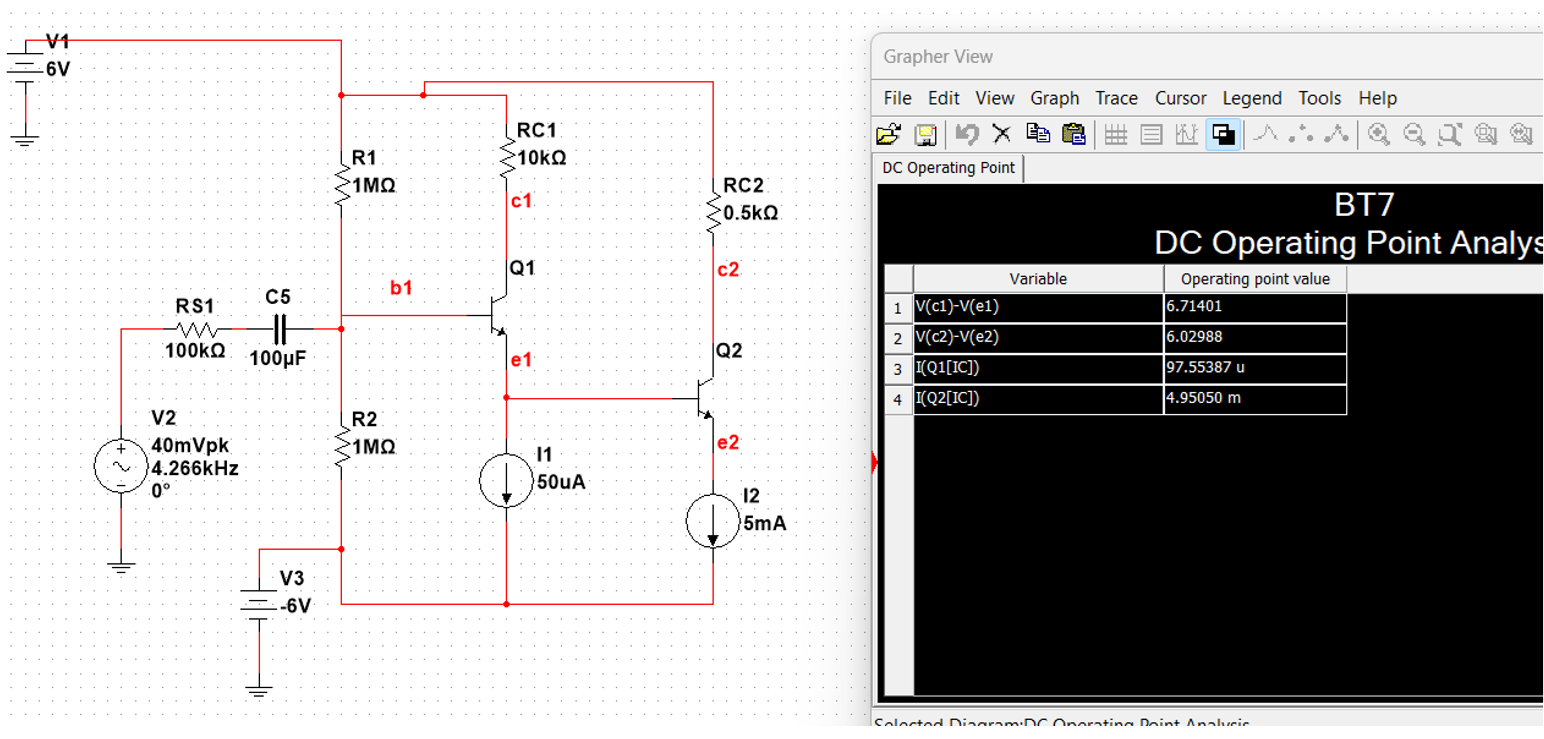
\includegraphics[width=.8\linewidth]{./my-chapters/my-images/Question7/a_ketqua_hinh.png}
\end{figure}

\answer{b}{Đặt nguồn $v_{s} = V_{m}\sin \left(  \omega t \right)$ có nội trở $RS = 100\,\textsf{k}\Omega$ vào mạch. Ngõ ra nối với tải $R_{L} = 1\,\textsf{k}\Omega$. Tìm $A_{v}$, $G_{v}$, $R_{in}$, $R_{out}$ của mạch. Biết nguồn dòng điện có điện trở nội là $10\,\textsf{k}\Omega$.}

Với đề yêu cầu thêm điện trở nội của nguồn dòng nên ta tiến hành giải lại điểm $Q_{1}$ và $Q_{2}$.

\begin{figure}[H]
	\centering
	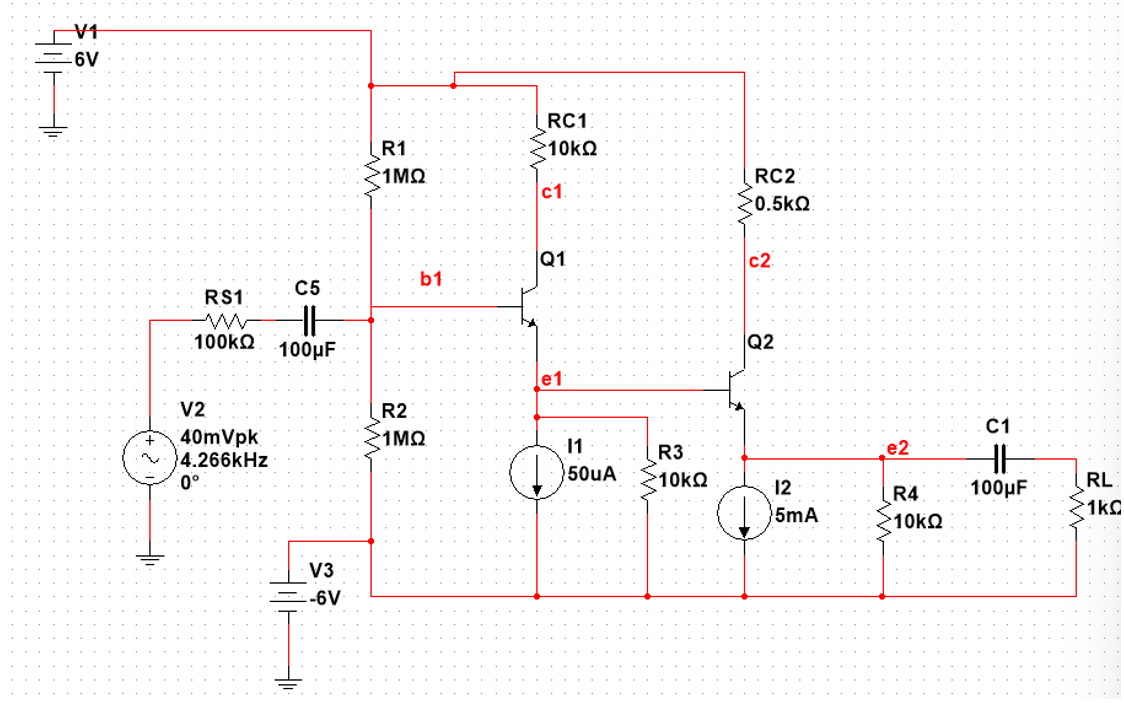
\includegraphics[width=.8\linewidth]{./my-chapters/my-images/Question7/b_giaiQ.png}
\end{figure}

\[ I_{E1} = 50\mu + \dfrac{V_{E1} + 6}{R_{3}} + \dfrac{I_{E2}}{\beta_{2} + 1} \]
Trong đó ta có, $I_{E2} = 5\,\textsf{mA} + \dfrac{V_{E2} + 6}{R_{4}} \quad \text{(1)}$
\[\Rightarrow I_{E1} = 50\mu\textsf{A} + \dfrac{VE_{1} + 6}{R_{3}} + \dfrac{5\,\textsf{mA}}{\beta_{2} + 1} + \dfrac{V_{E2} + 6}{R_{4}(\beta_{2} + 1)} \Rightarrow I_{E1} = 705\,\mu V_{E1} + 0.99\mu V_{E2} \quad \text{(2)}\]
\[ V_{B1} = V_{th} - I_{B1} R_{th} \Rightarrow V_{B1} = -I_{B1}R_{th} = - \dfrac{I_{E1}}{\beta + 1}R_{th} \quad \text{(3)}\]
Thế (2) và (3) ta có:
\[V_{B1} = -6.91 - 0.98V_{E1} - 0.0097V_{E2}\]
Với $V_{B1} - V_{E1} = 0.714\,\textsf{V}$, $V_{E1} - V_{E2} = 0.816\,\textsf{V}$

$\Rightarrow V_{B1} = -3.11 \,\textsf{V}\textsf{, }V_{E1} = -3.83\,\textsf{V} \textsf{, }V_{E2} = -4.64 \,\textsf{V}$ 

\noindent Thế vào (1) và (2),

$\Rightarrow I_{E2} =  5.136 \,\textsf{mA, }I_{E1} = 317\,\mu\textsf{A}$

Ta tiến hành chạy lại để đo DC cho mạch khi có thêm điện trở nội của nguồn dòng vào

\begin{figure}[H]
	\centering
	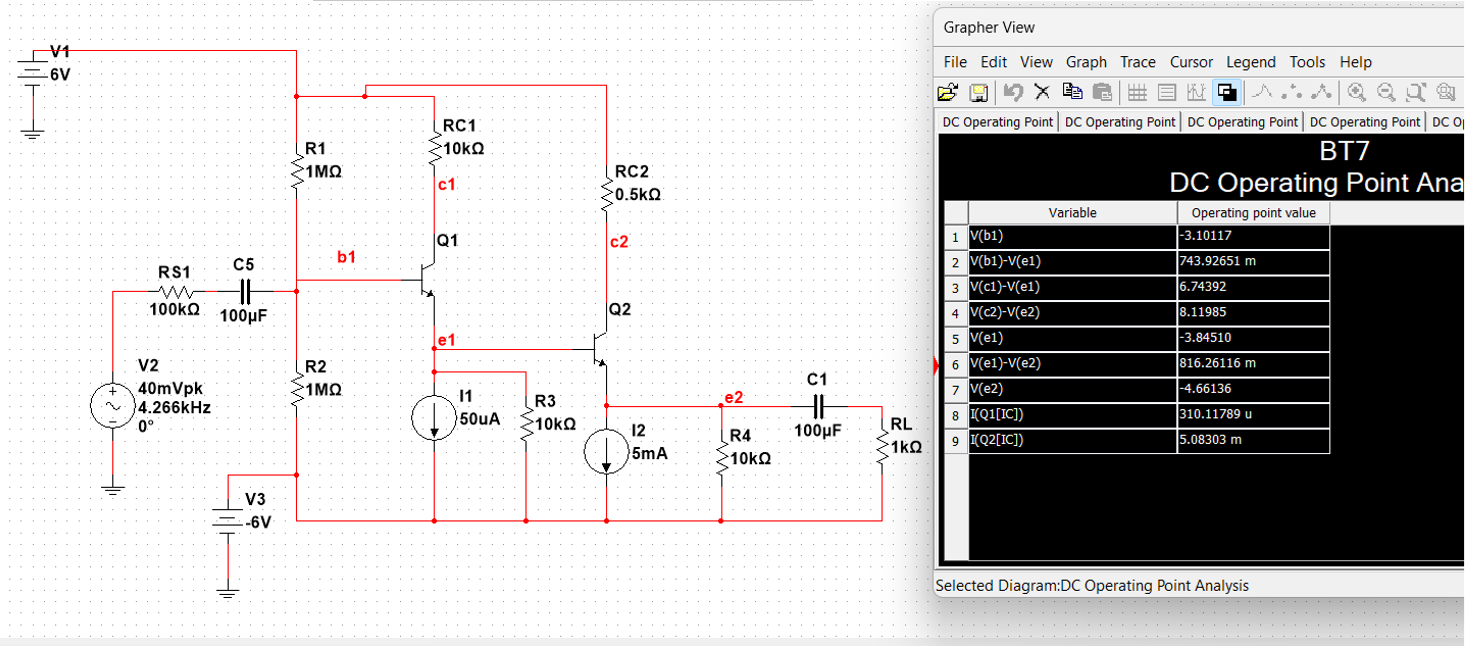
\includegraphics[width=.9\linewidth]{./my-chapters/my-images/Question7/b_Qnew.png}	
\end{figure}

Từ mô phỏng trên, ta lấy được thông số chính xác là \finalresult{I_{C1} = 0.31\,\textsf{mA, }I_{C2} = 5.08\,\textsf{mA}}.

Xét mạch hoạt động chế độ AC, ta có mạch tương đương như sau

\begin{figure}[H]
	\centering
	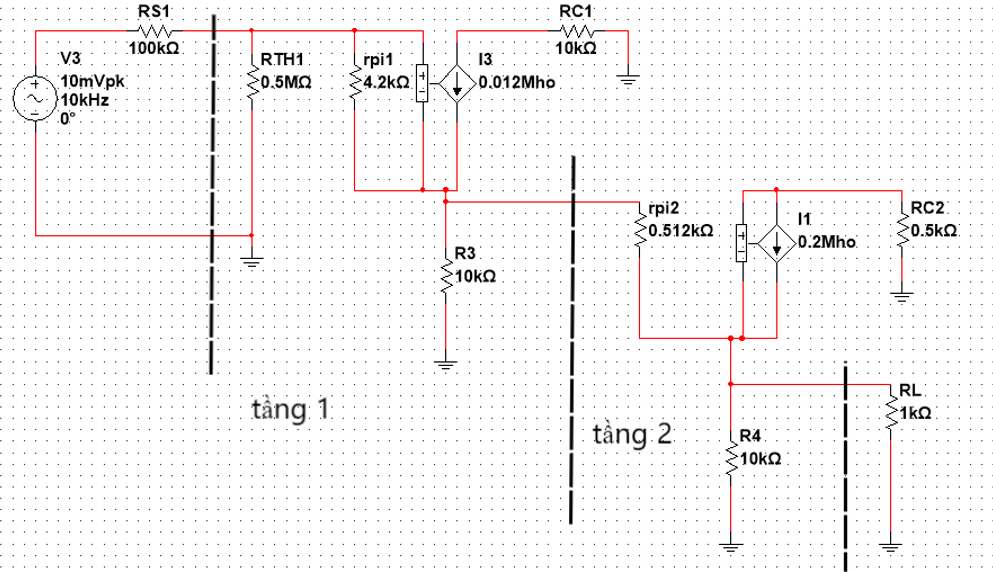
\includegraphics[width=.9\linewidth]{./my-chapters/my-images/Question7/b_machtuongduong.png}
\end{figure}

\begin{itemize}[label=+, leftmargin=2cm]
	\item $r_{\pi1} = \dfrac{V_T}{I_{B1}} = \dfrac{V_T \times \beta_1}{I_{CQ1}} = \dfrac{26 \times 50}{0.31} = 4.2\,\textsf{k}\Omega$
	\item $r_{\pi2} = \dfrac{V_T}{I_{B2}} = \dfrac{V_T \times \beta_2}{I_{CQ2}} = \dfrac{26 \times 100}{5.08} = 0.512\,\textsf{k}\Omega$
	\item $g_{m1} = \dfrac{I_{CQ1}}{V_T} = \dfrac{0.31}{26} = 0.012\,\textsf{S}$
	\item $g_{m2} = \dfrac{I_{CQ2}}{V_T} = \dfrac{5.08}{26} = 0.2\,\textsf{S}$
\end{itemize}

\begin{itemize}[label=-]
	\item Tầng 1
	\begin{itemize}[label=+, leftmargin=2cm]
		\item $R_{in1} = R_{TH1} // (r_{\pi1} + R_3(\beta_1 + 1)) 
		= 500\,\textsf{k} // (4.2\,\textsf{k} + 10\,\textsf{k}\times(50 + 1)) 
		= 253.5\,\textsf{k}\Omega$
		
		\item $R_{out1} = R_3 // \dfrac{r_{\pi1}}{(\beta_1 + 1)} 
		= 10\,\textsf{k} // \dfrac{4.2\,\textsf{k}}{51} 
		= 0.08168\,\textsf{k}\Omega$
		
		\item $A_{V1} = 
		\dfrac{R_3}{R_3 + \dfrac{r_{\pi1}}{(\beta + 1)}} 
		= 0.992\,\textsf{(V/V)}$
	\end{itemize}
	
	\item Tầng 2
	\begin{itemize}[label=+, leftmargin=2cm]
		\item $R_{in2} = r_{\pi2} + (\beta_2 + 1)R_4 
		= 0.512\,\textsf{k} + 101\times10\,\textsf{k} 
		= 1010\,\textsf{k}\Omega$
		
		\item $R_{out2} = R_4 // \dfrac{r_{\pi2}}{(\beta_2 + 1)} 
		= 10\,\textsf{k} // \dfrac{0.512\,\textsf{k}}{101} 
		= 5.067\,\Omega$
		
		\item $A_{V2} = 
		\dfrac{R_4}{R_4 + \dfrac{r_{\pi2}}{(\beta_2 + 1)}} 
		= \dfrac{1.5\,\textsf{k}}{1.5\,\textsf{k} + \dfrac{1.3\,\textsf{k}}{101}} 
		= 0.9995\,\textsf{(V/V)}$
	\end{itemize}
	
	\item Toàn mạch
	\begin{itemize}[label=+, leftmargin=2cm]
		\item \finalresult{R_{in} = R_{in1} = 253.5\,\textsf{k}\Omega}.
		\item \finalresult{R_{out} = R_{out2} = 5.067\,\Omega}.
		\item $A_{vo} = A_{v1} \times A_{v2} \times \dfrac{R_{in2}}{R_{out1} + R_{in2}} = 0.9907\,\textsf{(V/V)}$
		
		$\Rightarrow$ \finalresult{A_{vo} = 0.9907 \,\textsf{(V/V)}}.
			
		\item $A_v = A_{v0} \times \dfrac{R_L}{R_{out} + R_L} = 0.9857\,\textsf{(V/V)}$
		
		$\Rightarrow$ \finalresult{A_{v} = 0.9857\,\textsf{(V/V)}}.
			
		\item $G_v = A_v \times \dfrac{R_{in}}{R_{in} + R_S} = 0.707\,\textsf{(V/V)}$
		
		$\Rightarrow$ \finalresult{G_v = 0.707\,\textsf{(V/V)}}.
	\end{itemize}
	
	\item Kiểm tra kết quả
	
	\begin{figure}[H]
		\centering
		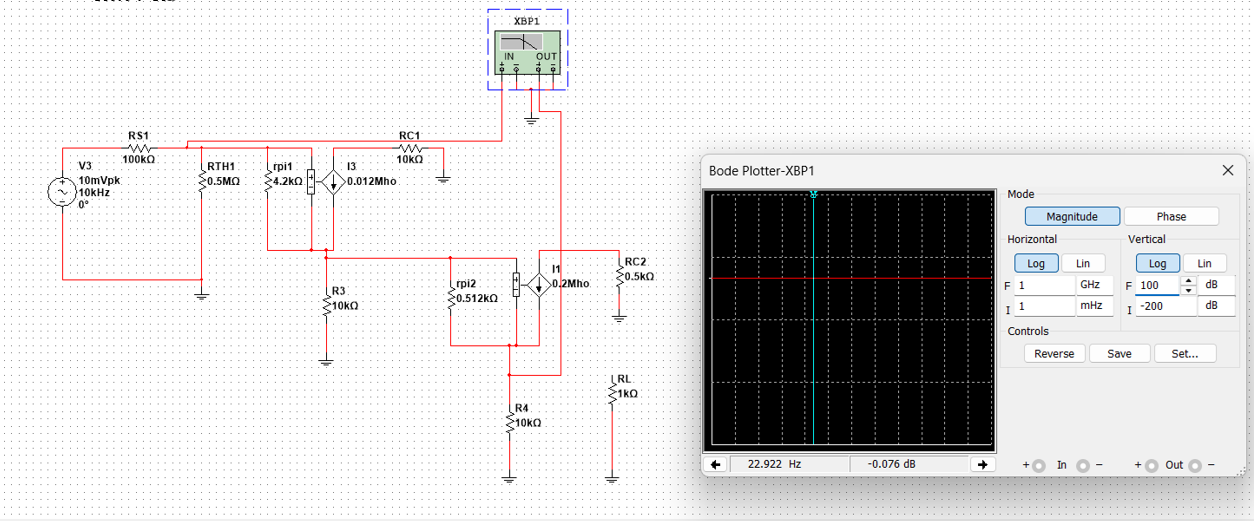
\includegraphics[width=.9\linewidth]{./my-chapters/my-images/Question7/b_avo_tuongduong.png}
		\caption{Đo $|A_{vo}| =-0.076 db = 0.991\,\textsf{V/V}$ (mô hình tương đương).}
	\end{figure}
	\begin{figure}[H]
		\centering
		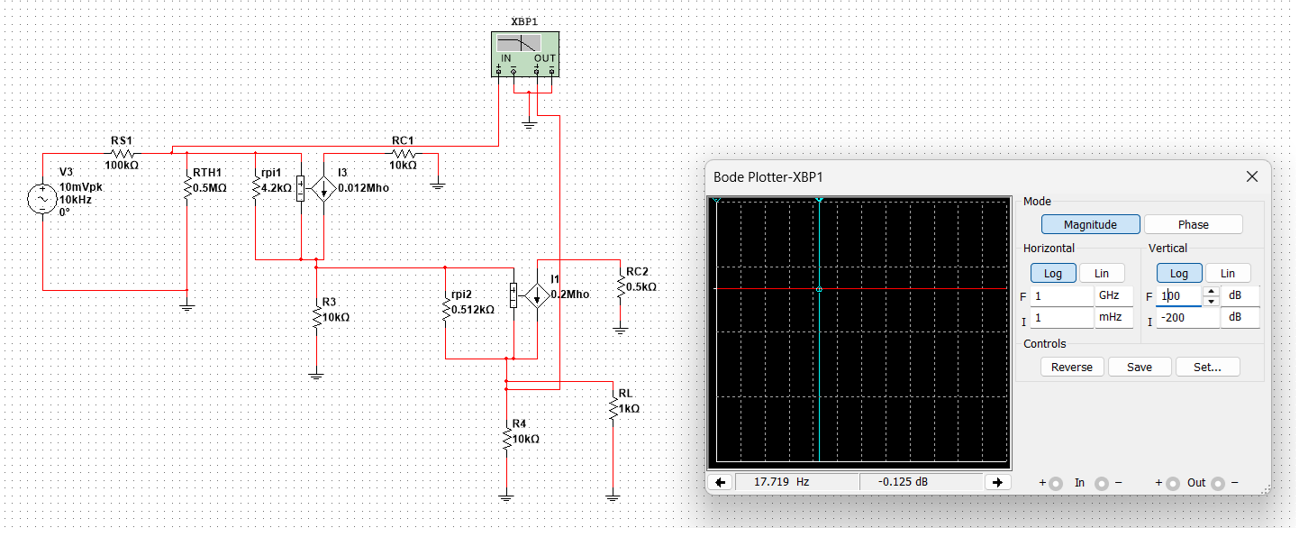
\includegraphics[width=.9\linewidth]{./my-chapters/my-images/Question7/b_av_tuongduong.png}
		\caption{Đo $|A_{v}| =-0.125 db  = 0.9857\,\textsf{V/V}$ (mô hình tương đương).}
	\end{figure}
	\begin{figure}[H]
		\centering
		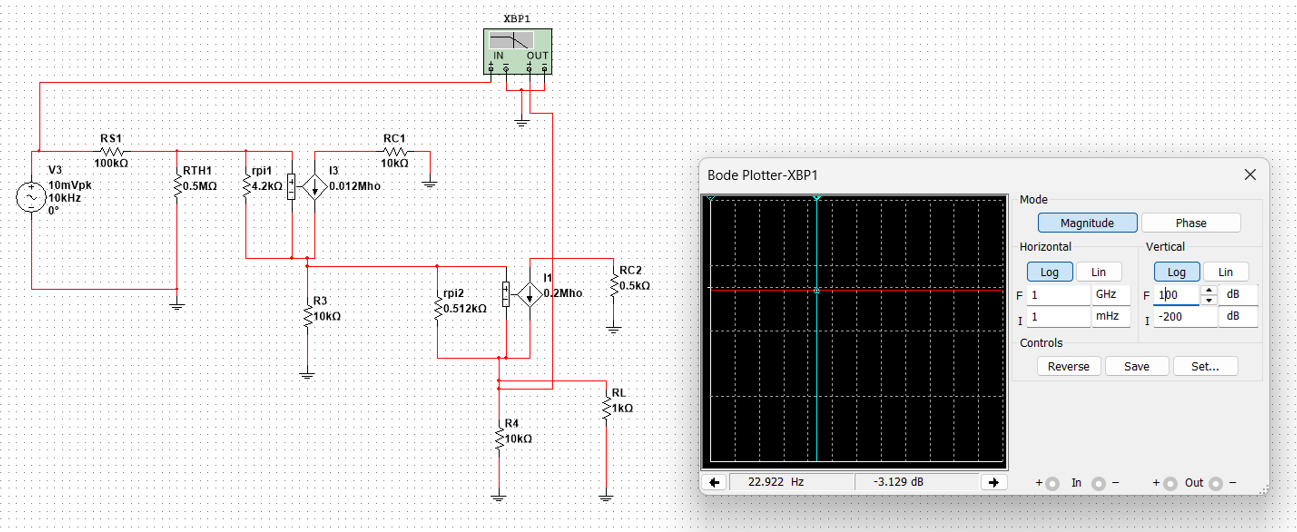
\includegraphics[width=.9\linewidth]{./my-chapters/my-images/Question7/b_gv_tuongduong.png}
		\caption{Đo $|G_{v}| =-3.129 db = 0.7\,\textsf{V/V}$ (mô hình tương đương).}
	\end{figure}
	\begin{figure}[H]
		\centering
		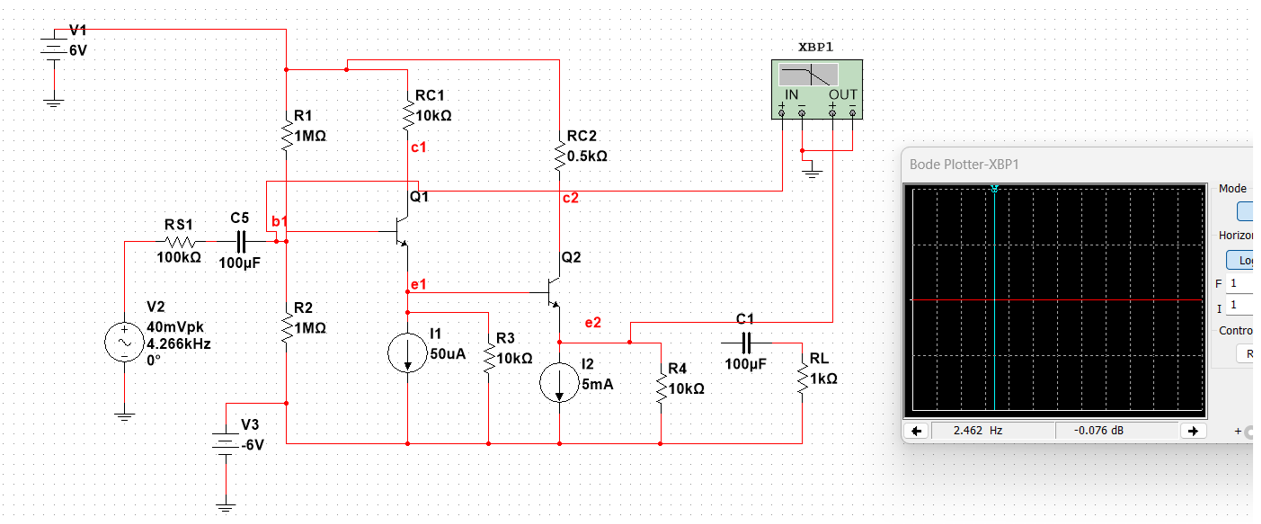
\includegraphics[width=.9\linewidth]{./my-chapters/my-images/Question7/b_avo_toanmach.png}
		\caption{Đo $|A_{vo}| =-0.076 db = 0.991\,\textsf{V/V}$ (toàn mạch).}
	\end{figure}
	\begin{figure}[H]
		\centering
		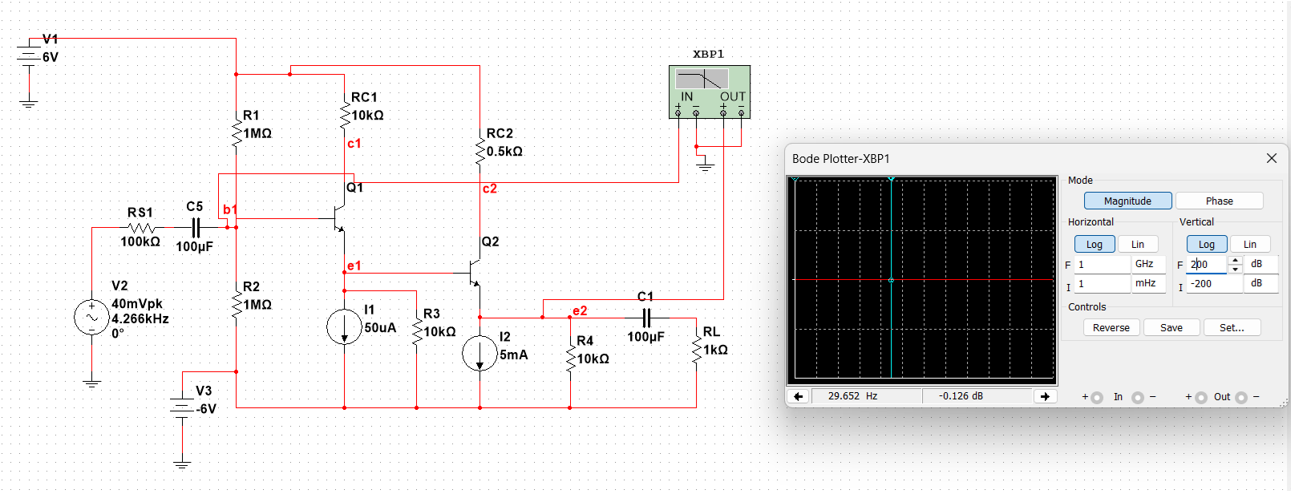
\includegraphics[width=.9\linewidth]{./my-chapters/my-images/Question7/b_av_toanmach.png}
		\caption{Đo $|A_{v}| =-0.126 db = 0.9856  \,\textsf{V/V}$ (toàn mạch).}
	\end{figure}
	\begin{figure}[H]
		\centering
		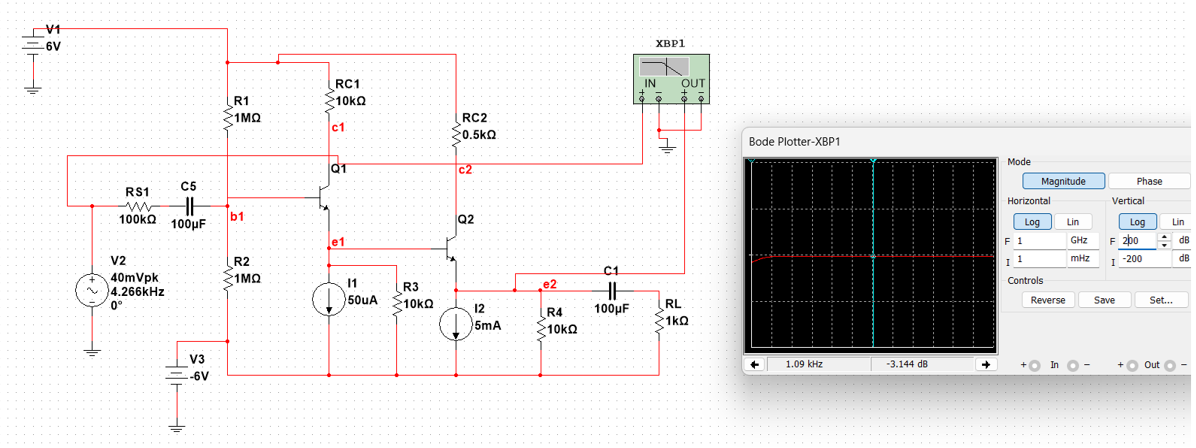
\includegraphics[width=.9\linewidth]{./my-chapters/my-images/Question7/b_gv_toanmach.png}
		\caption{Đo $|G_{v}| =-3.144 db = 0.7  \,\textsf{V/V}$ (toàn mạch).}
	\end{figure}
\end{itemize}

\answer{c}{Tìm biên độ lớn nhất của Vm để để vs là tín hiệu nhỏ ở cả hai tầng.}

Xét $Q_{2}$

\[ V_{CE} = 2V_{cc} - I_{C2} R_{C2} - (I_{C2} - I_{2})R_{4}\]
\[\Rightarrow V_{CE2} = 62 - 10.5\,\textsf{k}\times I_{C2}\]

\begin{figure}[H]
	\centering
	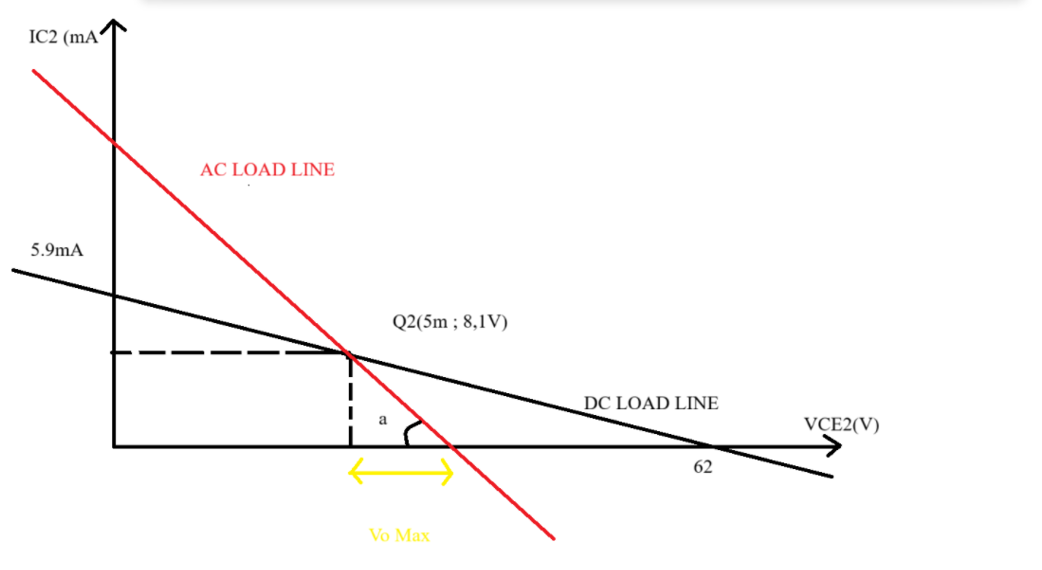
\includegraphics[width=.8\linewidth]{./my-chapters/my-images/Question7/c_hinh1.png}
\end{figure}

\[ \tan(\alpha) = \dfrac{1}{(R_{L}//R_{4}) + R_{C2}} = \dfrac{1}{1.4\,\textsf{k}}\]
\[\Rightarrow V_{o_{max}} = \dfrac{I_{CQ2}}{\tan(\alpha)} = 7 \,\textsf{V} \Rightarrow V_{sig_{max}} = \dfrac{V_{o_{max}}}{G_{v}\bigg|_{f = 1.09\,\textsf{kHz}}} = \dfrac{7}{0.7} = 10 (V)\]
$\Rightarrow$ \finalresult{V_{sig_{max}} = 10(V)}.

Dùng mô phỏng để quét từ $V_{sig_{max}}$ trở $x$ đến khi ngõ ra không méo dạng.

\begin{figure}[H]
	\centering
	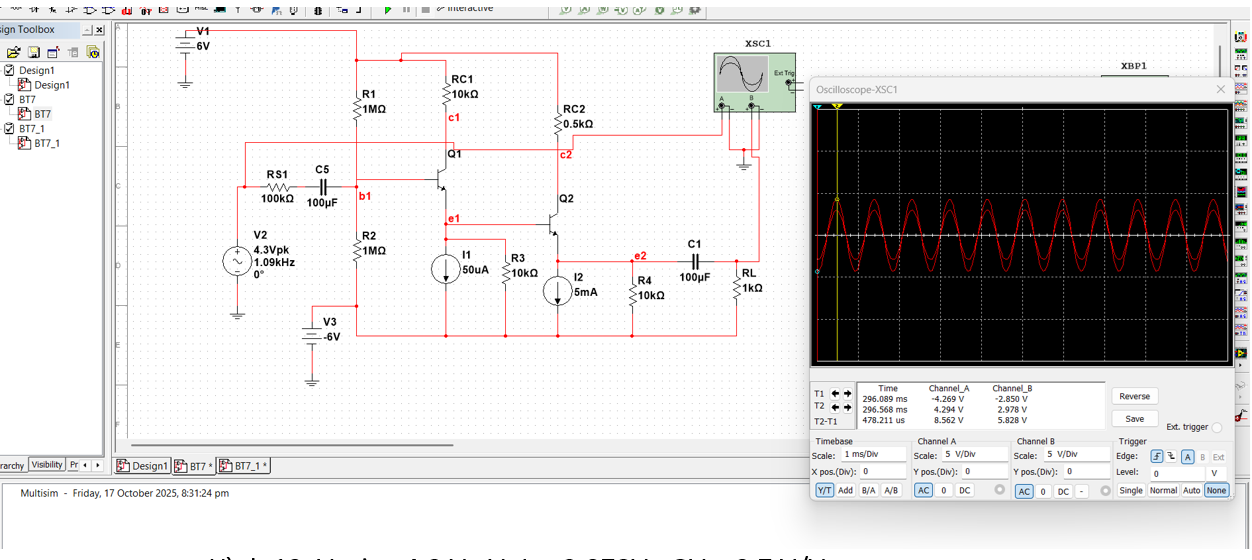
\includegraphics[width=.8\linewidth]{./my-chapters/my-images/Question7/c_hinh2.png}
	\caption{$V_{sig} = 4.3V$, $V_{pL} = 2.978V$, $G_{v} = 0.7\,\textsf{V/V}$.}
\end{figure}

\begin{figure}[H]
	\centering
	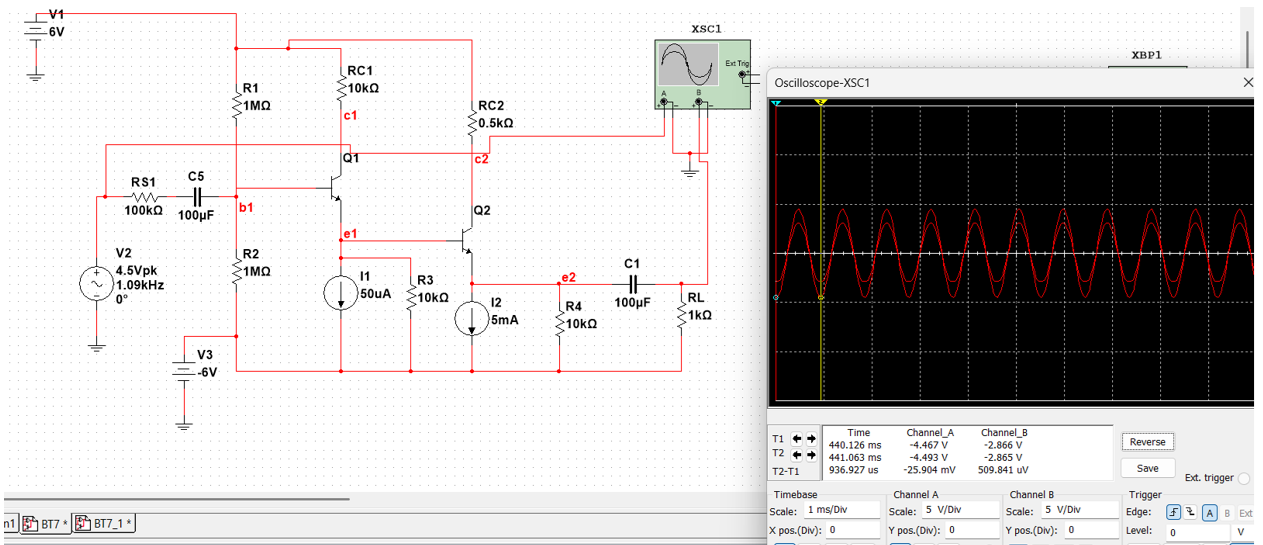
\includegraphics[width=.8\linewidth]{./my-chapters/my-images/Question7/c_hinh3.png}
	\caption{$V_{sig} = -4.5\,\textsf{V}$, $V_{pL} = -2.865\,\textsf{V}$, $G_{v} = 0.647\,\textsf{V/V}$ (ngõ ra bị xén dưới).}
\end{figure}

Vậy \finalresult{V_{m_{max}} = 4.5\,\textsf{V}}. 

